\documentclass[zihao = -4, linespread = 1.5]{ctexart}
\usepackage{mathandphy}
\usepackage{fancyhdr}
\pagestyle{plain}

\title{论}
\author{张睿}
\date{2021/04/15 \quad v0.6c}
\ctexset{
    abstractname = {\large{摘\quad 要}},
    bibname = {文\quad 献},
    contentsname = {\rmfamily\centerline{目\quad 次}},
    section = {
        format = \large\bfseries\sffamily
    },
    subsection = {
        format = \zihao{4}\bfseries\sffamily
    },
    subsubsection = {
        format = \normalsize\sffamily
    }
}

\begin{document}

\maketitle

\null
\begin{abstract}\normalsize
    车站连锁能够保证行车安全、提高运行效率,当下,在车站联锁系统中,
    计算机联锁已然成为主流。而计算机联锁培训系统就是用于计算机联锁教育培训的
    产品。而软件仿真则是最普遍的一种培训系统的模式。但传统的软件仿真计算机联锁
    培训系统存在着教学效率低、需要软件分发、软件运行环境限制、难以管理等问题。

    本设计使用IT行业内最新的软件设计技术,设计了一款基于Web、分布式、可扩展、
    高性能、高度灵活的计算机联锁培训系统,使用了极其高效的 Rust 程序设计语言,
    采用异步编程范式作为服务端,使用React.js和Two.js来渲染web端。
    设计为Web应用使得本设计不需要拘束于任何操作系统。
    并解决了传统软件计算机联锁培训系统的C/S模式的其他种种缺点,提高了培训效率。

    根据分布式的架构,本文使用了相应的技术来实现各层的各个模块,以及各个模块
    之间的耦合。在最后,对本设计进行了测试,以证明本设计实现了设计所要求的目标。
\end{abstract}
\textbf{关键字:} 分布式系统;Web应用;GraphQL;Rust程序设计语言;计算机联锁
\newpage

\twolines
\noindent\textbf{\large{Title}} ~ \uline{\large\hautengtitle\hfill}
\\
% \hangindent 4em \uline{\hautengtitle\hfill}

\renewcommand{\abstractname}{\flushleft\large{Abstract}}
\begin{abstract}\normalsize
    \noindent
    Computer-based interlocking has become the mainstream in station interlocking systems, which can ensure the safety of traffic and improve operational efficiency.
    The computer-based interlocking training system is a product used for computer-based interlocking education and training.
    Software simulation is the most common mode of training system. However, the traditional software simulation computer-based
    interlocking training system has problems such as low teaching efficiency, the need for software distribution, software operating environment restrictions,
    and difficulty in management.

    This design uses the latest software design technology within the IT industry to design a web-based, distributed, scalable, high-performance,
    and highly flexible computer-based interlocking training system that uses the extremely efficient Rust programming language,
    an asynchronous programming paradigm as the server side, and React.js and Two.js to render the web side.
    Designed for web applications makes this design not bound to any operating system.
    It also solves various other drawbacks of the C/S model of traditional software computer-based interlocking training system and improves the training efficiency.

    According to the distributed architecture, this paper uses the appropriate technology to implement each module of each layer and the coupling between each module.
    At the end, the design is tested to prove that it achieves the objectives required by the design.
\end{abstract}
\textbf{Keywords:} Distributed systems;Web application;GraphQL;Rust Programming Language;Computer-based interlocking
\newpage

\tableofcontents

\section{序论}
\subsection{研究背景与意义}
计算机联锁系统(CI)是综合运用计算机技术、网络通信技术和现代控制技术,
以电子信息传输方式集中操纵动力式道岔及色灯信号机等信号设备,从而实现控制车站的信号系统的功能的自动控制系统。
铁路车站是以建立进路的方式实现对列车、车列的运行控制。
计算机联锁系统通过计算机运算方式确保信号、道岔、进路间的相互关系正确,
满足各种车站、车场规模化运输作业的需要,能够保证行车安全,提高运输效率,改善劳动条件,
是车站信号设备控制系统的发展方向,是实现铁路现代化的重要基础之一。
联锁系统是铁路车站保证列车和车列正常和安全运行必不可少的核心基础设备。
而计算机连锁培训系统则是培训相关从业人员计算机连锁内容与相关操作的考试练习系统。
计算机连锁培训系统的目的在于:仿真模拟出现场的车站作业环境,能够达到练习、考试等培训功能,
通过练习功能、帮助学生深入学习计算机联锁,对计算机连锁的结构与操作工序逐渐的熟练,通过考试,
让教师能够对学生的水平有直观的判断与考察。提升计算机连锁教学的效率与品质。传统上,
计算机联锁培训通过视频教学、书本教学等培训手段,或者硬件模拟联锁逻辑实现,无法使仿真培训普及化以及并行化。
传统的计算机联锁教学相较于计算机联锁培训系统,更像是纸上谈兵,作为一门强实践性的技术,
计算机联锁培训系统能大大提高教育与学习的效率,已经是当今计算机联锁培训教育的首选教学工具。
若能结合联锁逻辑的纯软件模拟和web技术,则能让计算机联锁系统不再掣肘于空间与时间。
只要在可存取的互联网环境下,则可以处处进行计算机联锁的仿真学习。降低学习成本,提升学习效率。
摆脱了硬件仿真,则教学系统可以几近于零成本地部署在各处的服务器上,降低了安装部署的成本。
因此计算机联锁逻辑结合网络技术的应用,在计算机联锁培训领域内是十分重要的发展方向。

\subsection{国内外研究发展现状}
\subsubsection{国外现状}
国外对于计算机仿真培训系统采用了很多的技术手段来实现,因涉及很多学科,所以起步较早。
发达国家在上世纪八十年代就提出了相关的概念,并在十年内快速发展并取得良好的实用。
例如:英国铁路部门采用了计算机网络、计算机模拟器、信号模拟器等技术手段进行搭建系统,使用于模拟和培训;
美国主要采用计算机仿真技术、多媒体技术、网络技术等组成实训系统。
日本采用力学仿真及数据运算的同时还使用多媒体闭路电视进行直观培训。 

\subsubsection{国内现状}

在国内,计算机连锁培训系统主要分为以下三种形式:纯实物仿真培训、沙盘模拟仿真系统、纯软件的计算机联锁仿真培训系统。

纯实物仿真培训采用真实的信号机、钢轨、转辙器、轨道电路、列车等轨道交通信号设备作为仿真的表示层,
采用真实的计算机联锁软件进行仿真培训,这种培训方式的优点在于,最贴近实际作业环境,
能最真实的反应出学生在真实站场中可能遇到的各种场景和问题,表示直观,能体现出实际站场中信号设备和计算机联锁系统的耦合逻辑。
其缺点在于,成本耗费巨大,硬件调试困难繁杂,越复杂的车站便要越大的空间才能部署,培训难以并行化,车站毫无扩展性,
严重依赖硬件作为表示层,使培训流程严重受限于硬件状态。比如南京铁道职业技术学院内设有两个车站,相去1公里。

沙盘模拟仿真系统采用真实的信号机、钢轨、转辙器、轨道电路、列车等轨道交通信号设备作为仿真的表示层,
采用真实的计算机联锁软件进行仿真培训,这种培训方式的优点在于,拥有实物模型,能够直观的看到整个车站实际的状态,
比较贴近实际作业环境,占地面积小,整个车站只需要一间房间即可容下,相较于纯实物仿真而言成本低廉,但拥有纯实物仿真培训的大多数优点,此外,
由于可以将多个车站构建于一个沙盘上,每一个车站都能同时进行一人的培训。缺点:构建沙盘需要一定的成本,需要硬件调试,培训流程一定程度掣肘于硬件状态
,囿于列车的数量和位置,车站之间耦合性强,一个学生的培训流程会被其他学生的培训流程所影响,进而影响整个培训系统的效率。
整个系统能承载的学生和车站种类有限,可扩展性较差,如果沙盘上部署的车站不同,则无法进行标准化考试,只可作为练习使用。

纯软件的计算机联锁仿真培训系统采用完全软件模拟的表示层和联锁逻辑构建培训系统进行计算力联锁的仿真培训,
这种模式的优点在于没有任何的硬件电路,可用性强,可以通过升级软件等方式获得其他车站,而联锁逻辑是独立的通用模块无需更动,扩展性强,易于维护。
只需要计算机即可完成部署,不依赖大面积空间,成本低廉。不依赖硬件状态,可以不受限于其他车站的状态,软件可以复制,便于分发,
同一个车站可以分发给多个学生进行练习,能够实现并行化考试与练习,可以任意组合车站,不囿于物理的车站连接关系。易于设定权限组分别提升教师权限,
不掣肘于列车数量,可以随意增开列车排列进路。方便在考试前设定题目和评分标准,使所有学生同时使用相同的车站完成相同的任务方便标准化的考试,
产生有参考价值的考试成绩。

\section{需求分析}
uroj旨在设计一款高性能、可扩展、高并发、通用性计算机联锁培训系统。
通用性在于我们需要一款不拘束于某个具体车站的计算机联锁培训系统。本系统需要拥有对任意一车站进行
联锁培训的能力,可扩展性在于需要让用户可以自己定义车站。用户可以在自定义的车站上进行联锁培训,
并且要求定义过程简单易懂,不需要用户输入多余的内容。

若要满足这一点,传统的联锁表必然不符合,联锁表相当于枚举了整个车站的设备,车站规模越大,
联锁表就越复杂,而且如果要求用户上传联锁表用于联锁逻辑,则还要上传站场图用于渲染,但
显然的,站场图和联锁表描述的都是同一种事物--车站。由于这些问题,uroj选择了图论算法
来驱动联锁逻辑。而用户只需要编辑上传一个文件就能描述整个车站:包括各种设备之间的耦合关系
还有车站的地理布置。并使用这个车站来创建自己的计算机联锁模拟环境,这就是本设计的目标。


高性能在于作为一款web应用,尽量缩短相应时间、提升硬件利用效率,减少冗余。
高并发在于作为一款web应用,通过设计保证系统能够同时并行处理尽量多的请求。
\section{系统概览}
\subsection{系统架构}
为提高并发,提升应用性能,本案采用分布式系统设计,如图\ref{org} 所示,

\begin{figure}[htbp!]
    \centering
    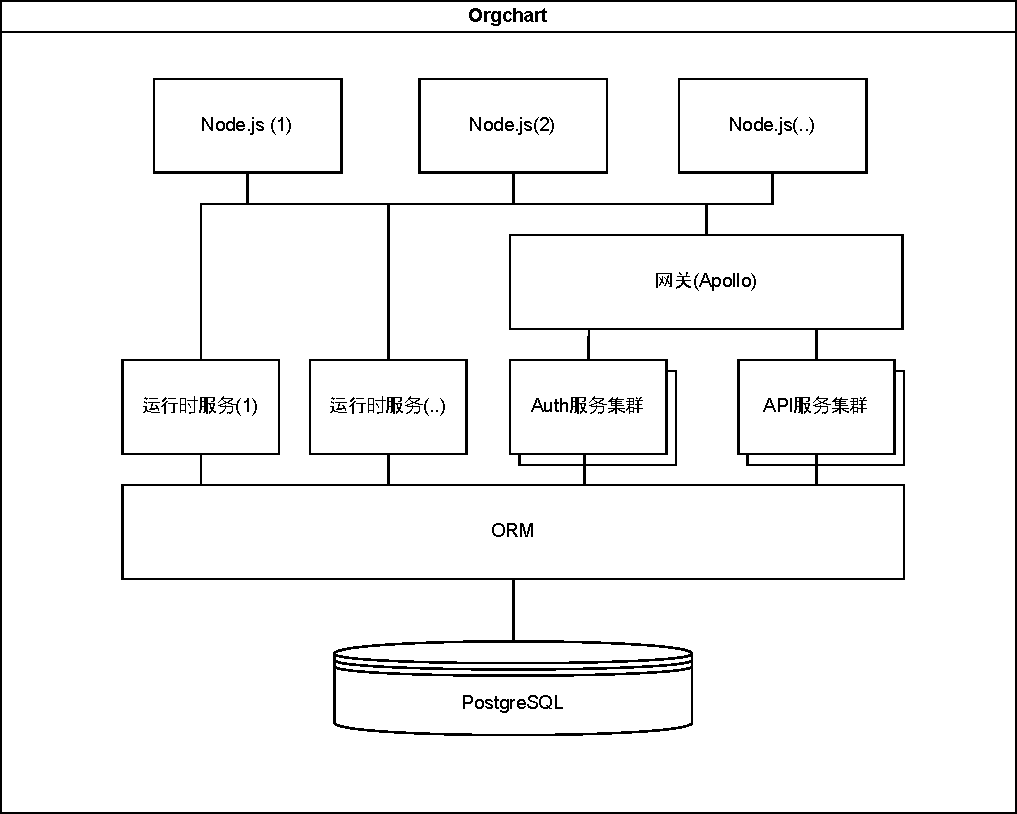
\includegraphics[width=0.95\textwidth]{figures/pdf/org.pdf}
    \caption{\label{org}系统架构组织图}
\end{figure}

本案符合非典型的web应用层次结构,分为表现层,接入层,业务逻辑层,数据访问层。
数据访问层采用名为 diesel 的 Rust crate 作为 ORM。
业务逻辑层分为Auth、API、Runtime等数个服务,每个服务都是独立的应用,可以横向扩展组成集群。
接入层使用 Apollo 作为 GraphQL 的网关,向外暴露所有的服务接口,还可以进行流量控制,但为了
支持运行时(Runtime)服务的“热插拔”,运行时服务并不会使用网关。
表现层使用 Node.js 作为 Web 的运行时,使用 React 作为 GUI 框架。
表现层和接入层、业务逻辑层使用 GraphQL 实现 Schema,使用 HTTP 和 WebSocket 协议通信,
并使用 actix-web 作为web服务端。


\subsection{生命周期与任务调度}
一个典型的练习实例生命周期由以下几部分组成
\begin{enumerate}[\indent i.]
    \item 创建车站
    \item 用户创建练习实例
    \item 初始化实例
    \item 访问实例
    \item 结束实例
\end{enumerate}

其中,创建车站就需要用到后文提到的车站描述文件,车站被创建后将存入数据库中。创建好车站后,就可以创建
这个车站的实例。实例是uroj的最终端功能,是用户与联锁逻辑交互的直接对象,也是uroj的业务核心。
一个用户的一次练习就是一个实例,一个用户的一次考试也是一个实例。

本案支持预约或称定时开始的实例,在开始之前若用户尝试在executor
初始化一个实例,就会报错。在GUI上,在开始时间之前,不渲染开始按钮,和后端的时间约束形成两层约束。
实例创建后同样也会被记录在数据库中,当时间到后用户就可以在创建实例时指定的executor上
初始化实例 -- executor从数据库中读入instance,并运行。
实例初始化后用户就可以在该实例中进行进路车辆的各种操作。
最后实例会被结束。

在uroj的架构中,runtime服务(后文也称为“执行器”)的作用是实例运行的容器。其提供了
实例运行所需要的环境(如联锁逻辑、车站拓扑关系分析等)一个容器可以同时让多个
实例在其中运行。因此得名运行时或执行器。正如上表所示,一个车站可以创造无限个实例,
这也是本设计通用性的一大体现。

一个典型的考试实例生命周期由以下几步构成
\begin{enumerate}[\indent i.]
    \item 创建车站
    \item 创建考题、考试
    \item 批量创建实例
    \item 初始化实例
    \item 访问实例
    \item 结束实例
\end{enumerate}

和练习实例不同之处在于,一场考试是有考题的。同一场考试中无论考试有多少,考题
都是相同的。通过班级结构,可以在配置考试实例时指定受验班级,系统自动为
班级所有的学生创建配置信息完全相同(即开始时间、结束时间、考题、车站等等)的实例。

本案正是通过对于考题、车站等配置信息的最高效复用以实现通用性的。
\section{服务端细节}
\subsection{API服务}
\subsection{Auth服务}
\subsection{Executor服务}
\subsection{实例组件}
\section{数据库架构}
\section{web端细节}
\section{网络通信}

\section{测试}


杀杀杀
\end{document}